\section{Measurement Tools, Environment, and Procedure}\label{sec:measurement}

\subsection{Environment}\label{sec:meas-env}
Following Castor's primer~\cite{castor2024primer}, Table~\ref{tab:env} lists what can affect the results; the Intel arm runs only if the laptop is repaired by 16~October.

\begin{table*}
\caption{Measurement environment.}
\label{tab:env}
\footnotesize
\setlength{\tabcolsep}{4pt}
\begin{tabular}{@{}p{0.11\textwidth}p{0.46\textwidth}p{0.38\textwidth}@{}}
\toprule
Element & Mac mini M4 (primary) & Intel Core Ultra~7 255H (conditional) \\
\midrule
CPU, memory & Apple M4 (\texttt{Mac16,10}): 4 P + 6 E cores; 16\,GB unified memory & 6 P + 8 E + 2 LP-E cores, no SMT; 32\,GB \\
Max.\ frequency & P 4464\,MHz, E 2892\,MHz (P mostly 3936\,MHz under all-core load) & P 5.1, E 4.4, LP-E 2.5\,GHz (Linux capacity 1024, 774, 312) \\
OS, power & macOS 27.0 (build 26A428); AC, Low Power Mode off & CachyOS Linux; AC \\
JDK, harness & OpenJDK 25.0.4.1 (Homebrew, LTS), JMH 1.37; shim: Apple clang 21 & same JDK and JMH \\
JVM flags & \multicolumn{2}{p{0.84\textwidth}@{}}{\texttt{-Xms2g -Xmx2g -XX:+UseG1GC -{}-enable-native-access=ALL-UNNAMED} (both platforms)} \\
Energy interface & IOReport ``Energy Model'' counters (C shim, FFM), refreshed at 100\,ms & RAPL via powercap (package, core, uncore, psys) \\
Frequency control & Apple's closed-loop performance controller; not user-settable, so logged & \texttt{intel\_pstate} with HWP, turbo on \\
\bottomrule
\end{tabular}
\end{table*}

\subsection{Energy Measurement}\label{sec:meas-energy}
\emph{Instrument.} The primary metric is \texttt{CPU\_Energy}, an IOReport counter with 1\,mJ resolution, verified to be the exact sum of the E and P clusters (ECPU + PCPU), whose split answers RQ3.2; the memory subsystem (DRAM, the AMCC memory controller, and DCS) is tested second on blocking workloads. A C shim called via the Foreign Function \& Memory (FFM) API reads all channels in-process, without root.

\emph{Synchronization and sampling rate.} A custom profiler for the Java Microbenchmark Harness (JMH) reads all counters in its before-iteration and after-iteration hooks and divides each iteration's energy by the operations completed. Nothing polls inside the measured region, avoiding the C-state suppression of high-frequency polling~\cite{raffin2025dissecting}; the sampling rate is two reads per iteration. On Intel it reads RAPL via powercap, correcting wraparound.

\emph{Refresh.} On macOS~27 the counters advance only at a privileged sampler's ticks (Section~\ref{sec:meas-pitfalls}), so \texttt{powermetrics} runs as root at 100\,ms as a refresher, also logging residency, frequency and thermal pressure. Each boundary read is therefore stale by at most about one refresh interval (106\,ms maximum in Table~\ref{tab:refresh}), about 2\% of a 5\,s window, and a canary check fails loudly if \texttt{CPU\_Energy} stalls for 0.5\,s or more.

\emph{Accuracy and precision.} RAPL has been validated against physical meters~\cite{khan2018rapl}; Apple's counters are unvalidated model estimates (Section~\ref{sec:threats}). Lacking a wall meter, we check the read path with AX3 (IOReport against \texttt{powermetrics} CPU power, which share one energy model) and linearity with AX4 (load scaling); neither validates absolute accuracy. Precision matters most for within-machine comparisons, and the staleness is under half the $\pm$5\% equivalence margin (Section~\ref{sec:planning-analysis}).

\subsection{Procedure}\label{sec:meas-procedure}
\begin{figure}
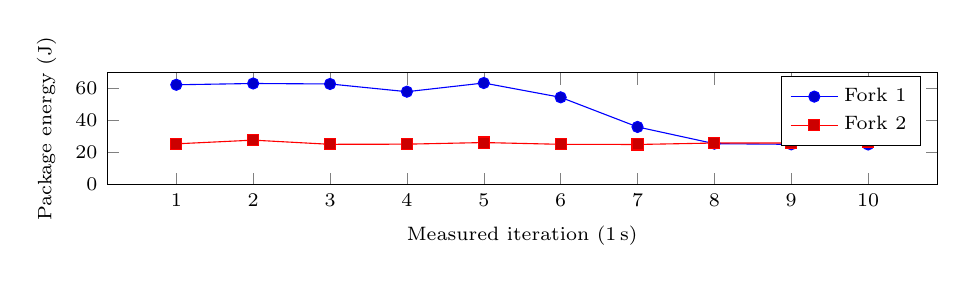
\begin{tikzpicture}
\begin{axis}[width=\columnwidth, height=3.0cm, xlabel={Measured iteration (1\,s)},
  ylabel={Package energy (J)}, ymin=0, xtick={1,...,10},
  legend style={font=\scriptsize, at={(0.98,0.97)}, anchor=north east},
  tick label style={font=\scriptsize}, label style={font=\scriptsize}]
\addplot+[mark=*] coordinates {(1,62.0)(2,62.8)(3,62.5)(4,57.7)(5,63.1)(6,54.2)(7,35.8)(8,25.4)(9,25.0)(10,24.9)};
\addplot+[mark=square*] coordinates {(1,25.3)(2,27.6)(3,25.0)(4,25.1)(5,26.1)(6,25.0)(7,24.9)(8,25.8)(9,25.8)(10,26.5)};
\legend{Fork 1, Fork 2}
\end{axis}
\end{tikzpicture}
\caption{Intel pilot, PT on CPU: package energy per 1\,s iteration falls from about 62\,J to 25\,J within fork~1 while time/op rises from 89 to 128\,ms; fork~2 starts in the low regime. Identical treatment, different power state.}
\label{fig:regime}
\Description{Line chart of package energy per one-second iteration for two forks: fork 1 starts near 62 joules and drops to about 25 joules after iteration 6, while fork 2 stays near 25 joules throughout.}
\end{figure}
\begin{table}
\caption{AX1: IOReport refresh vs.\ \texttt{powermetrics} interval.}
\label{tab:refresh}
\footnotesize
\begin{tabular}{@{}lrrrrr@{}}
\toprule
Interval (ms) & off & 1000 & 250 & 100 & 50 \\
\midrule
Updates in 6\,s & 0 & 13 & 47 & 111 & 208 \\
Max.\ gap (ms) & n/a & 1005.6 & 256.8 & 106.0 & 55.9 \\
\bottomrule
\end{tabular}
\end{table}
\begin{table}
\caption{Mac pilot, feasibility only ($p=8$, 3 forks $\times$ 5 $\times$ 5\,s): \texttt{CPU\_Energy}, medians of per-fork medians (W: mean); CV of per-fork J/op.}
\label{tab:pilot}
\footnotesize
\setlength{\tabcolsep}{2.5pt}
\begin{tabular}{@{}lrrrrrrrr@{}}
\toprule
 & \multicolumn{4}{c}{CPU} & \multicolumn{4}{c}{SLEEP} \\
\cmidrule(lr){2-5}\cmidrule(l){6-9}
 & ms/op & J/op & W & CV & ms/op & J/op & W & CV \\
\midrule
PT & 156.8 & 1.771 & 11.27 & 0.6\% & 16.61 & 0.0251 & 1.53 & 4.8\% \\
FP & 182.2 & 1.987 & 10.88 & 0.9\% & 458.6 & 0.0174 & 0.052 & 48.6\% \\
FJ & 182.2 & 1.974 & 10.84 & 0.7\% & 397.5 & 0.0080 & 0.057 & 116\% \\
VT & 154.8 & 1.767 & 11.40 & 0.9\% & 12.61 & 0.00035 & 0.027 & 2.1\% \\
\bottomrule
\end{tabular}
\end{table}
The 930 runs (the three workloads of Section~\ref{sec:planning-units}, 256 tasks per operation) follow a seeded random order in batches of about 40, each opened by a manifest (OS build, hardware, power settings, JDK, top processes), a quiet-machine gate, refresher start and a 60\,s idle baseline. \emph{Per run:} (1)~the gate requires $\geq$95\% CPU idle over 3\,s; (2)~one JMH invocation runs one fork of a cell with \mbox{\texttt{-f 1}} \mbox{\texttt{-wi 5}} \mbox{\texttt{-w 1s}} \mbox{\texttt{-i 5}} \mbox{\texttt{-r 5s}} \mbox{\texttt{-rf json}}; VT's carrier count is set per JVM (Table~\ref{tab:variables}), and BACKGROUND runs pass a \mbox{\texttt{taskpolicy -b}} wrapper to JMH's \mbox{\texttt{-jvm}} option; (3)~a cooldown of at least 10\,s lasts, on the Mac, until thermal pressure is ``Nominal''. On Intel, CPU-bound runs warm up for at least 60\,s (a heat-soak), beyond the boost phase of about 11\,s in the A1 pilot, so the measured window lies in the sustained power regime; the RAPL power-limit status is logged, and iterations crossing a regime change are flagged. Blocking workloads draw too little power to reach the limit.

\emph{Executions per trial.} A trial, one fork (Section~\ref{sec:planning-design}), has five 1\,s warmup iterations, as warmup times converged within two iterations in the Mac pilot, and five 5\,s measured iterations, which keep staleness at about 2\%.

\emph{Protocol and data.} All applications are quit, Do Not Disturb is on, Wi-Fi is off, Spotlight indexing is paused, the display sleeps, and \texttt{caffeinate} keeps the system awake. Each run yields a JMH JSON file; a schedule CSV (seed, timestamps), the \texttt{powermetrics} log, and per-batch idle baselines complete the data.

\subsection{Profiling}\label{sec:meas-profiling}
Java Flight Recorder (JFR, \texttt{profile} settings) attributes Java-level causes (thread starts, park and sleep, GC, hot methods); \texttt{powermetrics} records wakeups and cluster residency; on Intel, \texttt{perf stat} counts context switches, migrations, and cycles per core type. Each runs in separate passes (2 forks per selected cell), never during energy runs. JFR on the pilot's SLEEP workload at $p=8$ already exposes the mechanism: VT against PT showed 19 vs.\ 189,191 OS thread starts, 1 vs.\ 54 GCs, and 686 vs.\ 2,252 allocation samples (VT start events must be enabled explicitly).

\subsection{Familiarity with the Infrastructure and Pitfalls}\label{sec:meas-pitfalls}
Two pilots, the A1 pilot on Intel (RAPL, JDK~26.0.2, $p=8$, 2 forks $\times$ 10 $\times$ 1\,s) and a Mac feasibility pilot, exercised the pipeline end to end and exposed four pitfalls.

\emph{(1) Power-regime shift (Intel).} Under an identical treatment, package power dropped mid-fork (Figure~\ref{fig:regime}), and VT drew about 41\,W in fork~1 but 25\,W in fork~2, consistent with an unconfirmed PL2 to PL1 transition. JMH's fixed cell order confounded run order with power state, so our A1 CPU-bound figures (3.38 vs.\ 5.13\,J/op) averaged over both regimes. \emph{Response:} randomized fork order, a heat-soak warmup with power-limit logging and flagging (Section~\ref{sec:meas-procedure}), and AX7. On the M4, thermal pressure stayed ``Nominal'' in all 8094 pilot samples.

\emph{(2) Frozen and stale counters (macOS~27).} Counters update only at sampler ticks (Table~\ref{tab:refresh}): a 1\,s burn read without proper refresh gave 1100\,mJ, the \emph{prior} sample (1077\,mW $\times$ 1.01\,s), not the burn (8149\,mW). \emph{Response:} 100\,ms refresh, 5\,s windows, canary check.

\emph{(3) Sleep overshoot (macOS).} The analytic floor (Section~\ref{sec:planning-variables}) of FP/SLEEP at $p=8$ is nominally 320\,ms, yet the quiet Mac took 458.6\,ms (about 14.3\,ms per sleep wave) and a busy machine the same day 387\,ms (about 12.1\,ms): sleep latency depends on system activity, plausibly through timer coalescing. \emph{Response:} AX5 calibrates $d$, measured rather than nominal latency is reported, and SOCKET adds real I/O.

\emph{(4) Background load.} Idle CPU power was 0.020\,W on the quiet machine against 0.184\,W with everyday applications open (about 9$\times$). \emph{Response:} the quiet-machine protocol and gate.

\emph{Mac pilot.} Table~\ref{tab:pilot} supports no conclusion about which construct is greener (other FJ implementation, single $p$, three forks). Its CPU-bound cells are highly repeatable (Section~\ref{sec:planning-design}). Under SLEEP, CPU energy is at the noise floor (0.09 to 0.6\,J per 5\,s window for FP, FJ and VT, except one FJ window of 6.8\,J; idle-subtracted J/op of FJ and VT slightly negative, that is, within idle noise), unlike memory-subsystem energy (Section~\ref{sec:planning-design}). The refresher's overhead is at most 13\,mW (preliminary AX2), comparable to sleep-bound CPU power but constant across treatments.
